
\section{Experiments and results}
\label{sec:experiments-results}
NOTE: If CPU MIPS is high it is still OK to put the GPU actors on that
node.

We show the speedup obtained by our graph partitioning technique
compared to a single CPU allocation. Moreover, we compare our technique
with a heterogeneous bin-packing solution proposed in~\cite{mmar11}.

% Next, we compare our algorithm against two well known heuristic
% techniques Cross-Entropy~\cite{ssan05} and Simulated
% annealing~\cite{horsi06}. We chose these techniques, because they have
% already been successfully used for partitioning graphs onto
% heterogeneous architectures~\cite{ssan05}. Moreover, these two are the
% only techniques that perform reduced search space exploration and are
% able to produce decent results when auto-tuning compilers.

\subsection{Heterogeneous Bin Packing}

To determine how good our framework is, we compare it against an
adaptation of the well known heterogeneous bin packing solutions as
discussed by Teodor et al.~\cite{tcra11}. They adapt the well-known
\textit{Best First Decreasing (BFD)} heuristic, which works only for
homogeneous bins, to form the \textit{Adapted BFD (A-BFD)} heuristic
which works for heterogeneous bins. A small gist of the algorithm is as
follows.

Let $\mathcal{I}$ be the items to be accommodated into the bins and let
$\mathcal{K}$ be the set of bins available.  From the standpoint of the
mapping problem, $\mathcal{I}$ refers to the set of
\mbox{application-tasks ($V_t$)} and $\mathcal{K}$ refers to the PEs
($V_r$). Similar to the Knapsack problem~\cite{sski08}, by which A-BFD
is inspired, each element $i \in \mathcal{I}, \mathcal{K}$ has two
constraints on them represented by \mbox{$c_i$ (cost)} and $V_i$
(volume). % Right off the bat, this seems to be a significant advantage,
% our framework has over heterogeneous bin packing, as \textit{A-BFD} only
% works with two constraints whereas our framework poses no such
% restrictions.

\textit{A-BFD} proceeds to sort $\mathcal{I}$ according to
non-increasing order of their volume and sorts $\mathcal{K}$ according
to non-increasing order of the ratio $c_i/V_i$. Then, it proceeds to
allocate items from $\mathcal{I}$ into best bins $b \in \mathcal{S}$. A
``best" bin, i.e., the bin with maximum free space, is defined as the
bin volume minus the sum of volumes of the items loaded into it. % In the
% mapping problem setting, this becomes a double edged sword as it boils
% down to a single constraint solving problem giving higher priority to
% the second constraint (vector requirement of the application-tasks
% $T^i_1$ and vector capability of the resources $R^i_1$).

The post pass in \textit{A-BFD} chooses every bin that has atleast one
item allocated to it and tries to find an empty bin, that has a higher
or equal volume than the allocated volume on the chosen bin but also has
a lower cost. If it finds such an empty bin, then it transfers all the
items allocated to the chosen bin to the newly found empty bin which is
cheaper. One of the main advantages of \textit{A-BFD} is that it is very
fast with a best case complexity of $O(N_\mathcal{I})$ without the post
pass, where $N_\mathcal{I}$ is the number of items (number of tasks
$|V_t|$ in the application graph $G_t$). Including the post pass, the
best case complexity becomes $O(N_\mathcal{I} + N_\mathcal{K})$ where
$N_\mathcal{K}$ is the number of bins(number of PEs $|V_r|$ in the
resource graph $G_r$).


\begin{figure}[t!]
  \centering
  \includegraphics[angle=-90, scale=0.33]{./figures/binomial3d.eps}
  % \scalebox{0.4}{\input{./figures/binomial3d.eps}}
  \caption{Comparison of execution times of ``Our Framework" and ``Bin Packing"}
  \label{fig:binomial3d}
\end{figure}
